\question[3]
Schreibe eine Funktion \texttt{baum}, die den abgebildeten Baum zurückgibt.
Nutze dazu unsere Baum-Klasse.
Verschachtele die Baum-Aufrufe aus Lesbarkeitsgründen
höchstens einmal und gib den temporären Teilbäumen sprechende Namen.

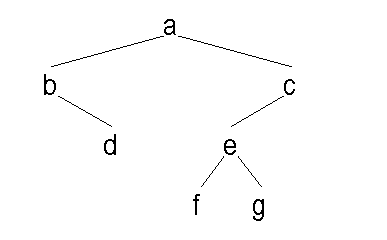
\includegraphics[height=4cm]{\pfad/Baum/Aufgaben/baumdef_03/baumdef_03.png}

\begin{solutionbox}{5cm}
\begin{lstlisting}
def baum():
    e = Baum('e',Baum('f'),Baum('g'))
    c = Baum('c',e, None)
    b = Baum('b',None,Baum('d'))
    a = Baum('a',b,c)
    return a
\end{lstlisting}
\end{solutionbox}
